\chapter{System Analysis and Design}
\label{Chapter3}

\section{Requirements Analysis}
\label{sec:requirements}

uMatter has four direct actors: the primary user, can be the teenager who
is seeking support for mental health or a close friend and family,
who tracks their wellbeing on the mobile application and owns every piece of
data they produce; the
therapist, working from the web dashboard; and the
administrator. Importantly, a teen may admit to their tracked record:
therapists, parents and close friends (other user accounts), the AI companion, all subject to the same explicit, scoped, revocable grants
(Section~\ref{sec: data}).

\begin{table}[htbp]
  \centering
  \caption{Key functional requirements and the objectives they realize}
  \label{tab:freq}
  \begin{tabular}{|l|p{8.2cm}|l|}
    \hline
    \textbf{ID} & \textbf{Requirement} & \textbf{Obj.} \\
    \hline
    FR1 & One-tap five-level mood check-in with optional context; journal
          with photos, mood calendar, and streaks. & O1, O6 \\
    \hline
    FR2 & Logs for sleep, nutrition and water, and breathing; step count is
          collected automatically and is the only passive signal. & O3, O4 \\
    \hline
    FR3 & Focus Mode prompts a check-in roughly every 90 minutes during
          waking hours, silent during user-configured Quiet Hours. & O2 \\
    \hline
    FR4 & The AI companion grounds its replies in the user's own tracking
          data if and only if the user has granted it access. & O5, O9 \\
    \hline
    FR5 & Guided breathing and meditation, and a Treasure Box of saved
          positive memories, routed to by logged emotion; an emergency
          area reachable in one tap from anywhere. & O6, O7 \\
    \hline
    FR6 & Therapist discovery, appointment booking, video consultation, and
          clinical notes; tracked data visible to a therapist only under an
          explicit, scoped, revocable grant. & O8, O9 \\
    \hline
    FR7 & Friend and parent connections with real-time chat; a connection by
          itself exposes no tracked data. & O9 \\
    \hline
    FR8 & Domain events produce push, email, and in-app notifications to the
          affected parties. & O2, O8 \\
    \hline
  \end{tabular}
\end{table}

\begin{table}[htbp]
  \centering
  \caption{Key non-functional requirements}
  \label{tab:nfreq}
  \begin{tabular}{|l|p{8.2cm}|l|}
    \hline
    \textbf{ID} & \textbf{Requirement} & \textbf{Obj.} \\
    \hline
    NFR1 & Privacy by default. No tracked data is visible to any
           audience without an active grant, enforced server-side so a
           compromised client cannot bypass it. & O9 \\
    \hline
    NFR2 & Stateless security. RSA-signed JWTs validated locally by
           every service against a published JWKS key. & O10 \\
    \hline
    NFR3 & Integrity under concurrency. Concurrent bookings of the
           same slot must not both succeed; retried requests are not applied
           twice. & O8 \\
    \hline
    NFR4 & Independent evolvability on modest infrastructure. Each
           service develops, deploys, and migrates independently, and the
           full platform runs on a single cloud virtual machine. & O10, O11 \\
    \hline
  \end{tabular}
\end{table}


\section{Overall Architecture}

\begin{figure}[htbp]
    \centering
    % Assuming your main.tex is at the root directory, you need the full path
    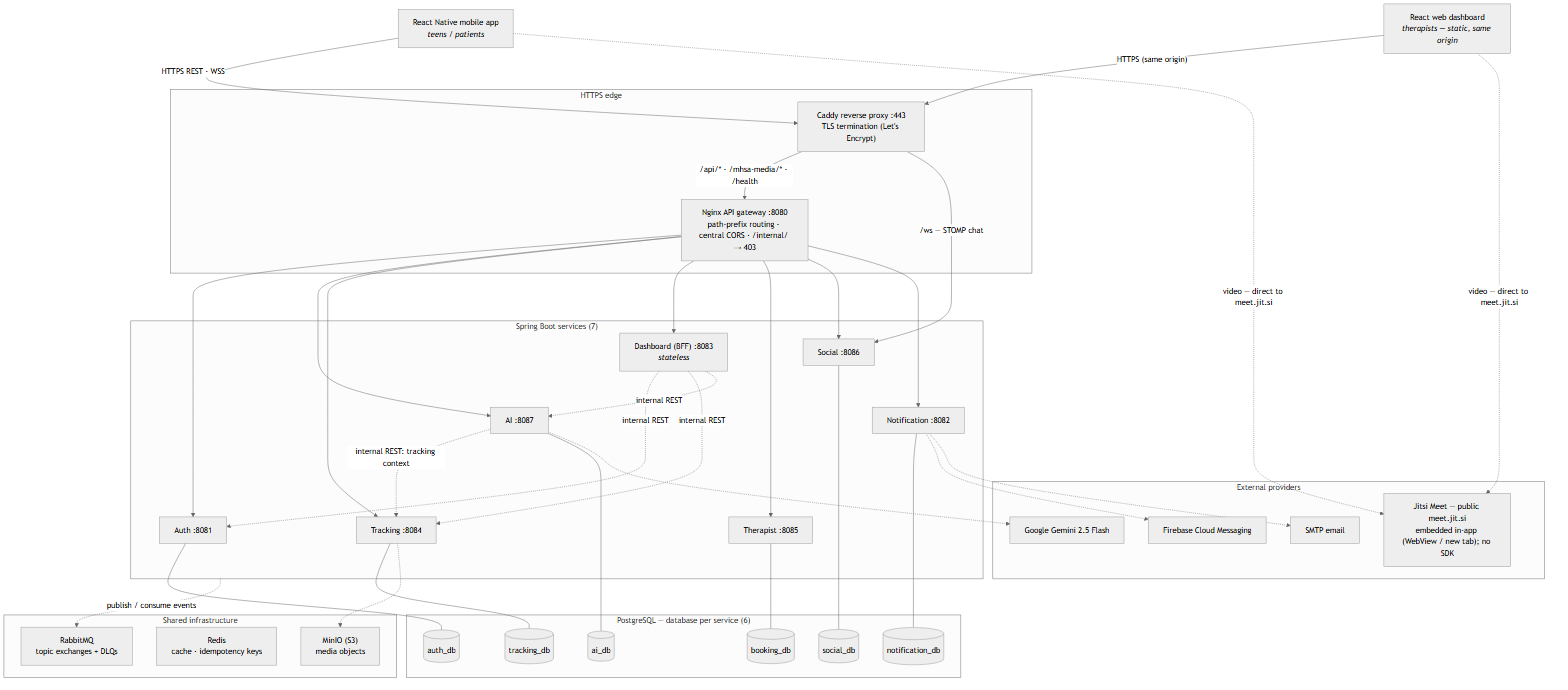
\includegraphics[width=\textwidth]{Chapter3/images/ch3-overall-architecture.png}
    \caption{The overall microservices architecture of uMatter.}
    \label{fig:ch3_overall_architecture}
\end{figure}

uMatter follows a microservices architecture: independently deployable Spring Boot services sit behind a single Nginx API gateway, which is the only entry point reachable by the two client applications - a React Native mobile app for teenagers/patients and a React web dashboard for therapists. The gateway is responsible for routing requests to the correct backend service and for terminating HTTPS at the edge of the system.

This decomposition is not free, and for a two-person academic project the
choice deserves justification. We accept the operational overhead of seven
deployables, a message broker, and per-service databases in exchange for
two things. First, independent lifecycles, which are not hypothetical here:
the services live in separate repositories, evolving without
coordinated upgrades. Second, each service is scoped to a single functional area, can be developed, deployed, and scaled independently, and owns its own data.

This decomposition follows the pattern described by Newman~\cite{2021-Newman-Microservices}, synchronous request/response interactions between services and clients use REST-style HTTP APIs~\cite{2000-Fielding-REST}; workflows that are naturally asynchronous, such as sending a notification after an event happens elsewhere in the system, are handled through RabbitMQ instead~\cite{RabbitMQ}.

\section{Service Decomposition}

The backend is organized into seven services, summarized in Table~\ref{tab:services}.

\begin{table}[ht]
\caption{uMatter backend services and their responsibilities}
\label{tab:services}
\begin{center}
\begin{tabular}{ |L{2.6cm}|L{9.5cm}| }
 \hline
 \textbf{Service} & \textbf{Responsibility} \\
 \hline
 Auth & User registration/login, JWT issuance and refresh, JWKS key publication, role management \\
 \hline
 Tracking & Mood, sleep, and journal entry storage; the source of truth for a user's self-reported well-being data \\
 \hline
 AI & Manages conversations with the AI companion, grounding responses in the user's own tracking data \\
 \hline
 Dashboard & Aggregates tracking data into summaries and visual trends for the user \\
 \hline
 Therapist & Therapist discovery/matching, appointment booking, video consultation session management, clinical notes \\
 \hline
 Social & Peer relationships (friends) and real-time chat over STOMP/WebSocket \\
 \hline
 Notification & Consumes domain events and delivers push (FCM), email, and in-app inbox notifications \\
 \hline
\end{tabular}
\end{center}
\end{table}


\section{Data Architecture}
\label{sec: data}

uMatter follows a database-per-service pattern: each backend service owns a private PostgreSQL database, and no service reaches directly into another service's schema. Cross-service data needs are satisfied either through a synchronous API call to the owning service or through an asynchronous event, never through shared tables. This keeps each service free to evolve its own schema without coordinating a migration across the whole system, at the cost of needing an explicit strategy (API calls or events) for any data that spans services.

Two supporting stores complement PostgreSQL:

\begin{itemize}
\item \textbf{Redis} is used for caching and for idempotency keys, so that a retried request (for example, a client retry after a network timeout) is not applied twice.
\item \textbf{MinIO}, an S3-compatible object store, holds binary media such as profile photos and any files attached to journal entries or clinical notes, keeping large binary payloads out of the relational databases.
\end{itemize}

To prevent synchronous bottlenecks when one service frequently requires data owned by another, the system utilizes an event-driven replication strategy via RabbitMQ topic exchanges. As illustrated in Figure~\ref{fig:ch3-replication-events}, the architecture maintains four primary replication streams: the Therapist API replicates auth-owned therapist profiles; the Tracking Service maintains a local replica of data access grants (serving as the consent gate for patient data); the Auth service replicates patient-therapist assignments; and the Social service listens for active assignments to automatically provision direct chat channels between patients and their therapists.

To ensure data integrity and fault tolerance across these asynchronous boundaries, all replication consumers implement a strict set of resilience patterns. Consumers utilize manual acknowledgments and operate as a single consumer per queue to maintain reliable processing. Message failures are routed to a Dead Letter Exchange and Queue (DLX/DLQ) for debugging and replay. Furthermore, to safely handle duplicate message deliveries, consumers enforce database-watermark idempotency based on an \texttt{occurredAt} timestamp. Finally, to guarantee eventual consistency and recover from any prolonged messaging outages, a nightly reconciliation process synchronizes the replica tables against an internal snapshot provided by the data owner.

\begin{figure}[htbp]
    \centering
    
    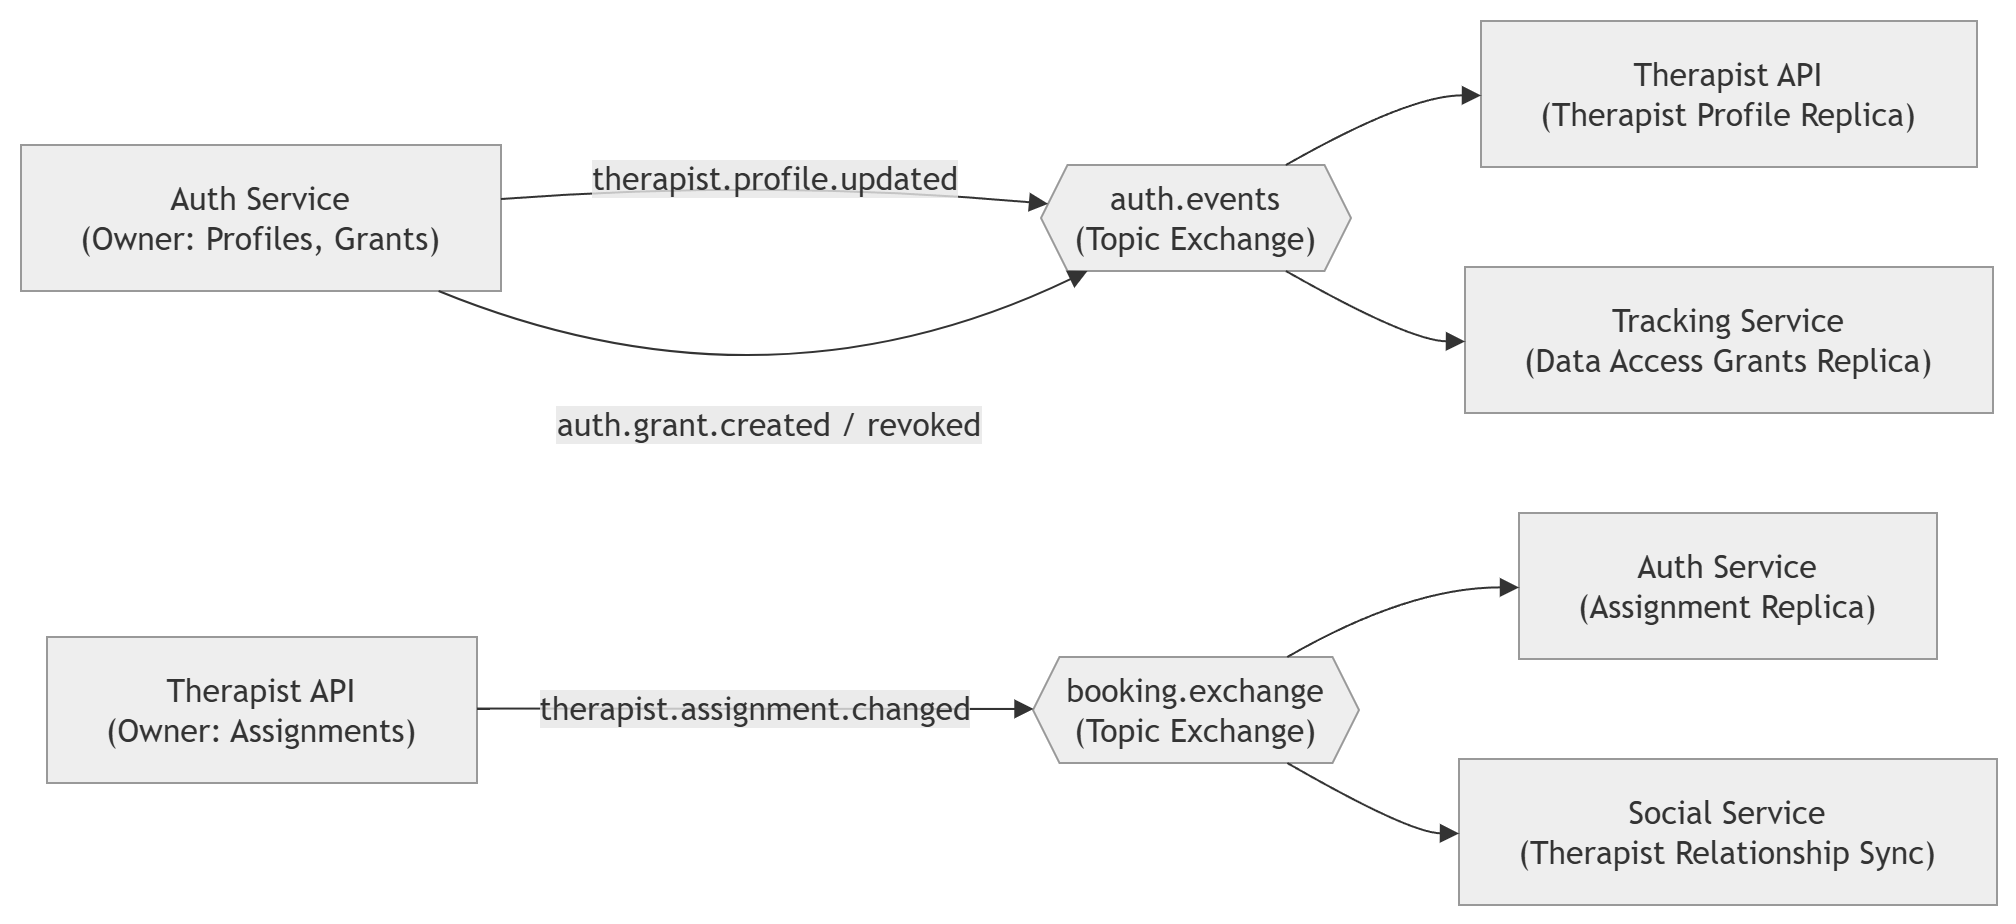
\includegraphics[width=0.8\textwidth]{Chapter3/images/ch3-replication-events.png}
    \caption{The four replication streams}
    \label{fig:ch3-replication-events}
\end{figure}

\section{Authentication, Authorization, and Data Sharing}
\label{sec:datasec}

\begin{figure}[htbp]
    \centering
    
    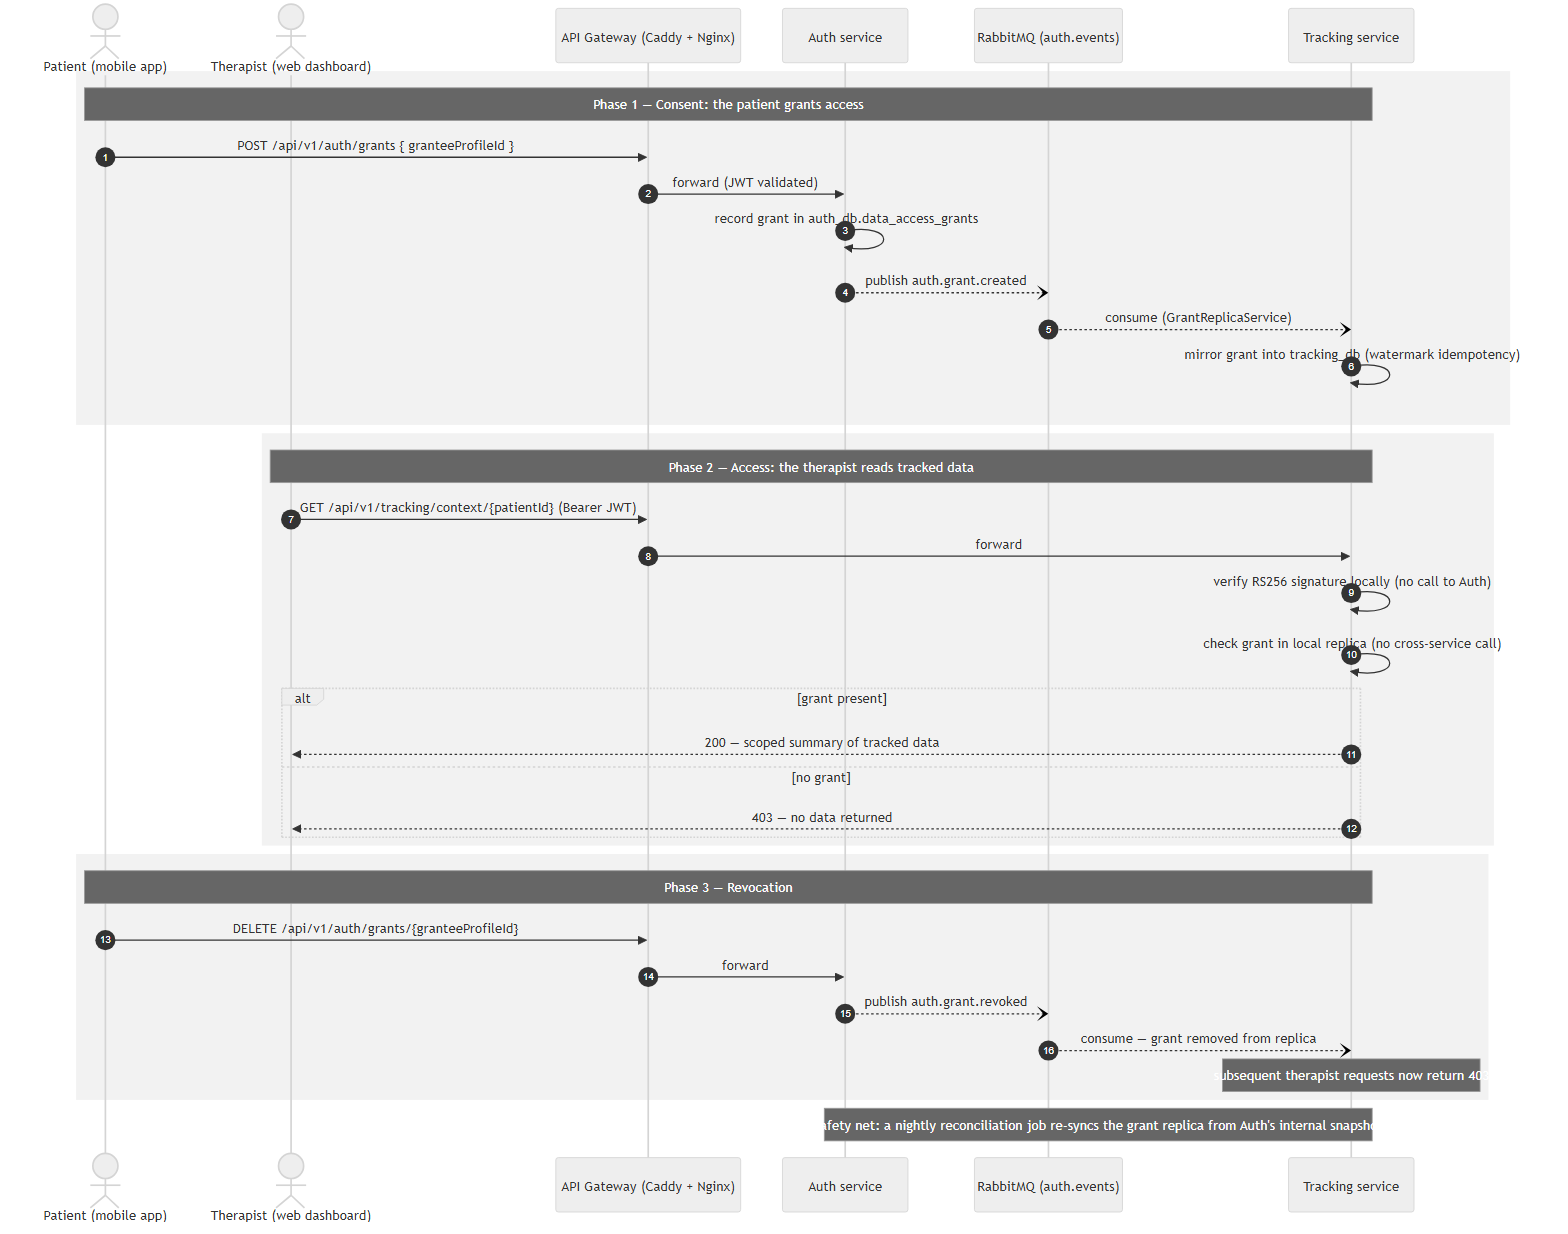
\includegraphics[width=\textwidth]{Chapter3/images/ch3-permission-grant-flow.png}
    \caption{A sequence diagram of a permission-checked data access.}
    \label{fig:ch3-permission-grant-flow}
\end{figure}

Authentication is stateless: the Auth service issues JSON Web Tokens signed with an RSA private key, following RFC 7519~\cite{2015-RFC7519-JWT}, and publishes the corresponding public key through a JWKS endpoint. Every other service validates incoming tokens locally against this published key, so no service needs to call back to Auth (or share a session store) simply to authenticate a request. Roles embedded in the token (teen/patient, therapist, admin) drive coarse-grained authorization at the gateway and service level.

Fine-grained authorization is handled by a permission-based data sharing model, which is central to uMatter's design goal of not exposing sensitive tracked data by default. A user's mood, sleep, food, journal, step, and breathing records are private to that user unless the user explicitly grants another party access. A grant names a \emph{set of tracking categories} it covers, so a user may share, for example, their sleep and nutrition but withhold their journal, carries a thirty-day expiry, and is revocable at any time. Enforcement lives at the Tracking service boundary: every read of a category is gated on an active, unexpired grant whose scope set includes that category, checked against a locally replicated copy of the grants (Section~\ref{sec:events}) rather than left to the client application, so that a compromised or misbehaving client cannot bypass it. The same mechanism serves every audience uniformly: a therapist, a parent, a friend, and the AI companion are all grantees enforced by identical code.

Service-to-service calls follow a two-tier trust model. User-facing APIs
(\texttt{/api/**}) always require a valid JWT, validated locally by the
receiving service. Internal APIs (\texttt{/internal/**}) --- such as the
Tracking endpoint the AI service calls to assemble conversation context, or
the grant snapshot the Tracking service pulls from Auth during nightly
reconciliation --- do not carry the user's token; the caller passes the
subject's profile identifier explicitly. These endpoints are protected by
network topology instead: they are reachable only on the private container
network, and the gateway refuses any external request whose path begins with
\texttt{/internal/}. Asynchronous messaging is likewise authenticated at the
broker with per-deployment RabbitMQ credentials. The trade-off is that any
process on the internal network is trusted; mutual TLS or per-service
credentials would remove that assumption and are noted as future hardening,
but within a single-host deployment where the internal network is not shared
with third-party workloads, perimeter trust is a proportionate design.

\section{AI Companion}

\begin{figure}[htbp]
    \centering
    
    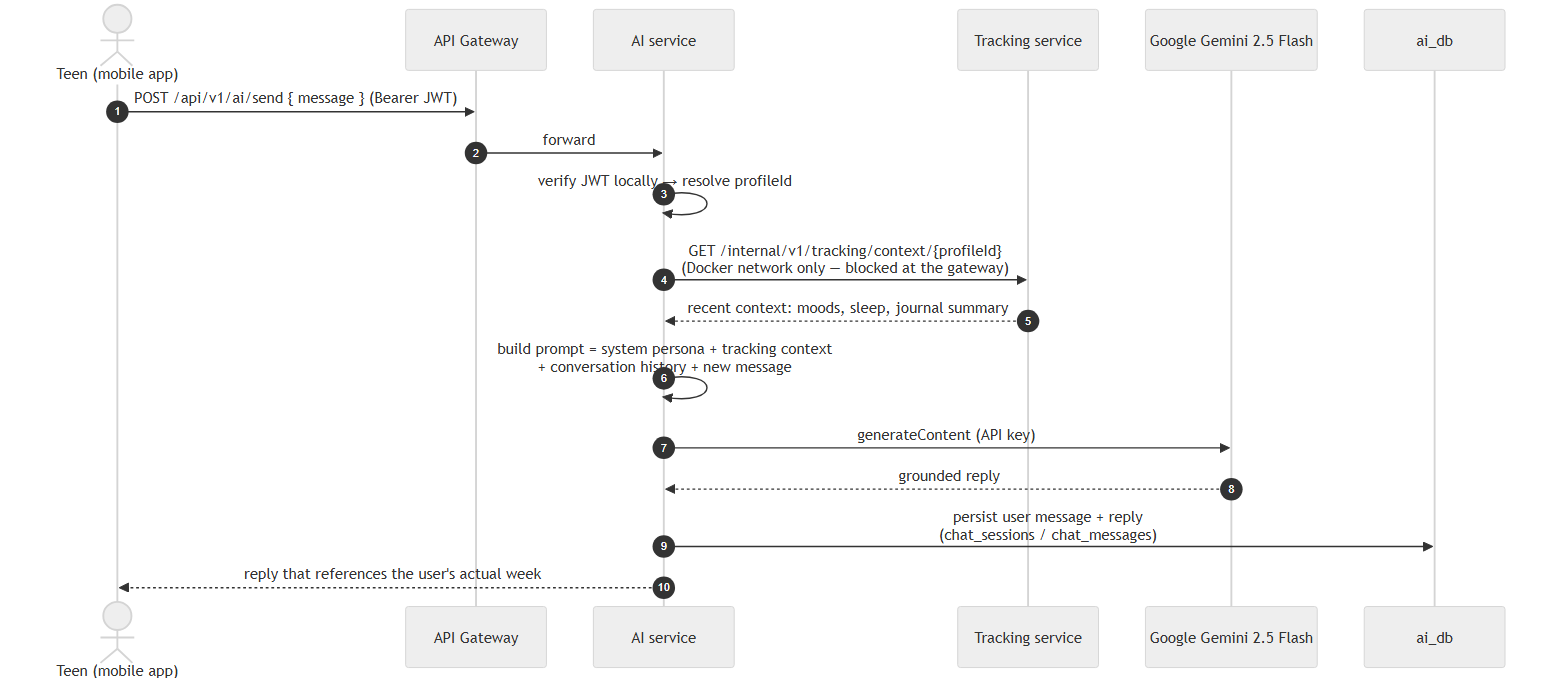
\includegraphics[width=\textwidth]{Chapter3/images/ch3-ai-grounding.png}
    \caption{A sequence diagram of AI grounding}
    \label{fig:ch3-ai-grounding}
\end{figure}

The AI companion is implemented in the AI service. It retrieves the user's recent tracking summary from the Tracking service and includes it as context when calling Google's Gemini 2.5 Flash model~\cite{2024-Gemini-TechReport}. Grounding the model in the user's own data lets the companion respond to something concrete (``you logged trouble sleeping three nights this week'') rather than only offering generic supportive text. Crucially, this retrieval is gated by the same data-access grant model as every other audience (Section~\ref{sec:datasec}): the AI service holds no standing access, and the Tracking service returns context only when the user has an active grant to the reserved AI-companion principal. Consent is off by default --- a user who has not opted in still receives a companion, just one that converses without personal grounding --- and can be revoked at any time from the chat screen, after which the next reply is ungrounded.

Two safeguards run on every message before and around this grounding, and both are deliberately narrow. First, user messages pass a lightweight keyword guardrail: a message matching a small list of Vietnamese self-harm or violence phrases short-circuits the model entirely and returns a fixed response directing the user to emergency hotlines, rather than being sent to Gemini. Second, personally identifying details (emails, phone numbers, and self-introduced names) are scrubbed from the message, history, and context before they leave the platform, and chat contents are encrypted at rest. What the AI service deliberately does not do is any form of clinical risk assessment or automated escalation to a third party --- no scoring, no alerting a therapist or family member --- which is left out of scope, as discussed in Chapter~\ref{Chapter5}, pending the clinical collaboration such a feature would require. The keyword guardrail is a within-conversation safety redirect, not a diagnostic claim.

\section{Professional Workflows}

The Therapist service implements the professional-facing half of the platform: it matches users to therapists based on stated preferences and availability, handles appointment booking, manages Jitsi Meet video consultation sessions~\cite{Jitsi} for the appointment, and stores clinical notes that a therapist records after a session. Appointment booking is a point of particular concern for data integrity, since two concurrent booking requests for the same therapist and time slot must not both succeed; the resolution of this issue is described in Chapter~\ref{Chapter4}.

\section{Peer and Family Connection}
\label{sec:social}

The Social service manages friend relationships and real-time chat over
STOMP/WebSocket. A parent participates through the same mechanism as anyone
else: a parent account (distinguished only by an account type recorded at
registration) connects to their child as a friend, and the connection itself
exposes no tracked data whatsoever.

Visibility is governed exclusively by the grant model of
Section~\ref{sec:datasec}. From a friend's profile screen, a teen may grant
that friend, who is a parent or peer, a scoped access to their tracked data,
issued with a 30-day expiry and revocable at any time; the friend then sees
mood and wellbeing summaries for the granted window, and nothing after
revocation or expiry. There is deliberately no privileged parental path and
no automatic alerting: our baseline study found that an automatic crisis
alert to family was rejected outright as pressure to perform a better mood
than the one being felt, and the professionals we consulted advised that
family connection be explicit and user-controlled. A parent therefore knows
exactly what their child has chosen to show them, which is the point.

\section{Event-Driven Messaging}
\label{sec:events}

\begin{figure}[htbp]
    \centering
    
    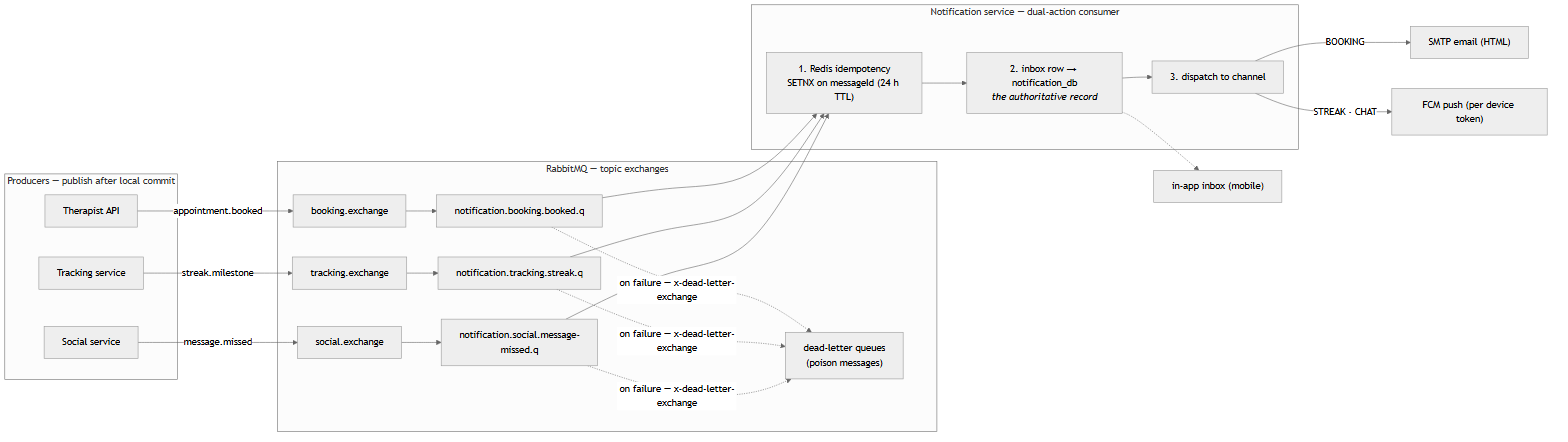
\includegraphics[width=\textwidth]{Chapter3/images/ch3-notification-events.png}
    \caption{An event-flow diagram}
    \label{fig:ch3-notification-events}
\end{figure}

RabbitMQ~\cite{RabbitMQ} connects services that should not depend on each other synchronously. 

Table~\ref{tab:events} catalogs the domain events. Each queue is paired with
a dead-letter queue, so a message that repeatedly fails processing is parked
for inspection rather than blocking the consumer.

\begin{table}[htbp]
  \centering
  \caption{Domain events exchanged over RabbitMQ}
  \label{tab:events}
  % The X columns will automatically expand to fill \textwidth evenly.
  \begin{tabularx}{\textwidth}{|>{\raggedright\arraybackslash}X|l|l|>{\raggedright\arraybackslash}X|}
    \hline
    \textbf{Event} & \textbf{Producer} & \textbf{Consumers} & \textbf{Purpose} \\
    \hline
    \texttt{auth.\allowbreak grant.\allowbreak created}, \texttt{auth.\allowbreak grant.\allowbreak revoked} & Auth &
      Tracking & Replicate consent grants so enforcement is local to the
      data owner \\
    \hline
    \texttt{therapist.\allowbreak profile.\allowbreak updated} & Auth & Therapist &
      Keep the therapist directory in sync with account profiles \\
    \hline
    \texttt{therapist.\allowbreak assignment.\allowbreak changed} & Therapist &
      Social, Auth & Propagate the active patient--therapist assignment
      (e.g.\ opening the corresponding chat) \\
    \hline
    \texttt{appointment.\allowbreak booked} & Therapist & Notification & Fan out booking
      confirmations as push, email, and in-app notifications \\
    
    \hline
  \end{tabularx}
\end{table}

\section{Self-Care Feature Design}
\label{sec:selfcare}

\textbf{Focus Mode.} Check-in prompts are scheduled entirely on the device:
enabling Focus Mode pre-schedules a batch of local notifications at roughly
90-minute intervals (about three days' worth), and the queue is topped up
whenever the application is opened. The Quiet Hours window (22:00--07:00 by
default, user-configurable) is applied at scheduling time and stored only on
the device.

\textbf{Streaks and the mood calendar.} Streaks are computed server-side by
the Tracking service as entries arrive, per tracking category, and the mood
calendar is a read view over the same store. Cross-category trend summaries
shown on the home screen are assembled by the Dashboard service, which reads
Tracking through an internal aggregation API rather than owning any data of
its own.

\textbf{Treasure Box.} Stored positive memories are Tracking-service records
whose photo attachments live in MinIO, and they are surfaced along the
emotion-routing path of Section~\ref{sec:requirements} (FR5): a user logging
sadness is offered their saved memories, a user logging anger a breathing
exercise.

\textbf{Emergency path.} The emergency-support area is a dedicated screen
reachable from anywhere in the application in one tap. It is intentionally
static client-side content, support and hotline resources render.

\section{Deployment Topology}

\begin{figure}[htbp]
    \centering
    
    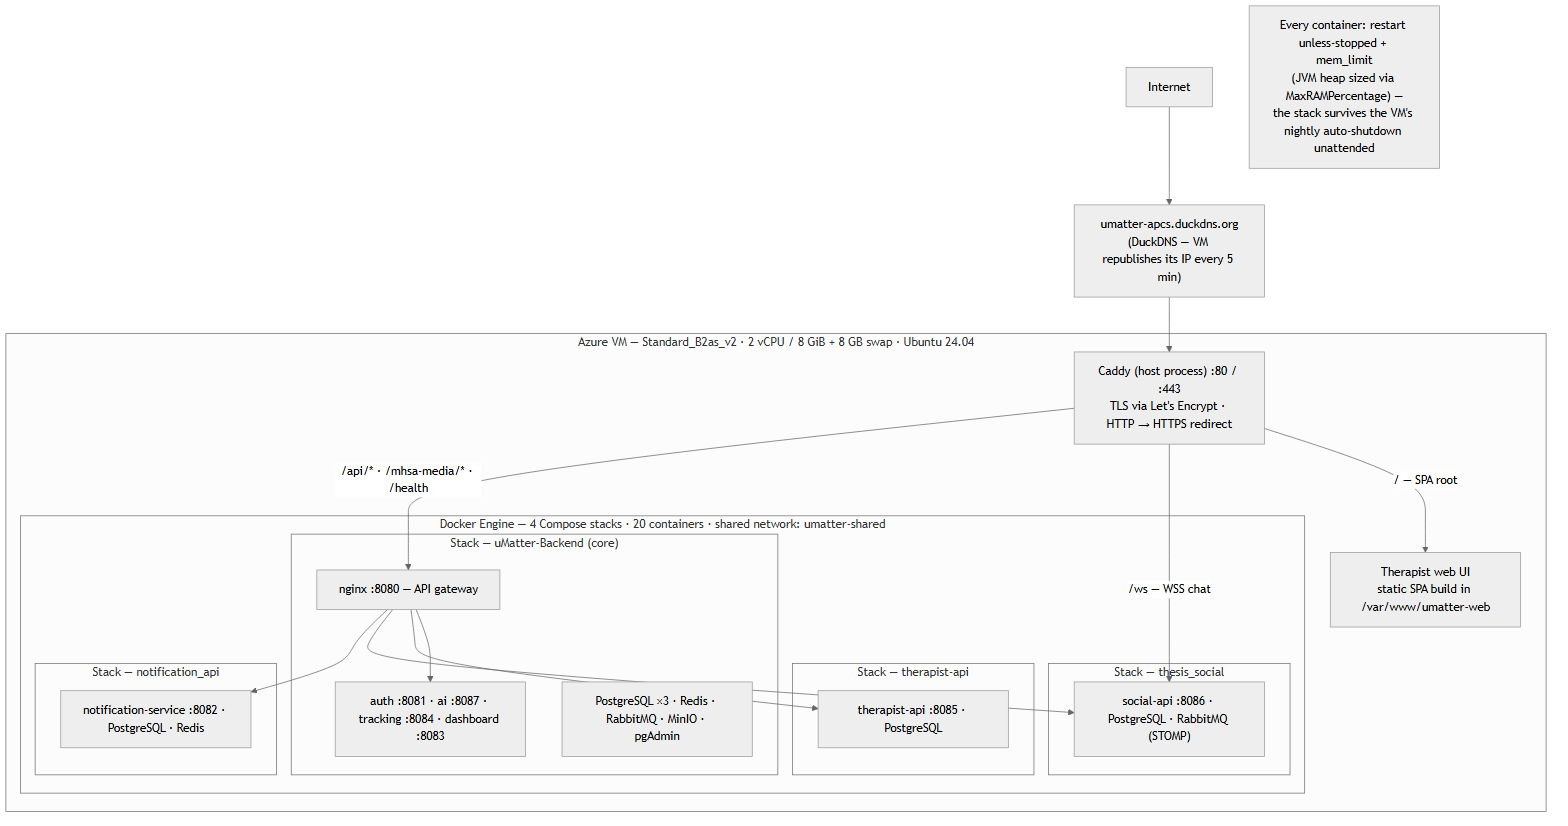
\includegraphics[width=\textwidth]{Chapter3/images/ch3-deployment-topology.png}
    \caption{A deployment diagram}
    \label{fig:ch3-deployment-topology}
\end{figure}

All services are packaged as Docker containers~\cite{Docker} and orchestrated with Docker Compose, grouped into stacks by repository. The full system - Spring Boot services, PostgreSQL instances, RabbitMQ, Redis, MinIO, and supporting tools such as pgAdmin - runs on a single cloud virtual machine, fronted by a reverse proxy that terminates HTTPS. The concrete deployment used for evaluation, including the migration between cloud providers, is described in Chapter~\ref{Chapter4}.
